\chapter{Theoretical Background}

\section{Single-particle dynamics in electron storage rings}
Ultra-relativistic beams of electrons are injected into the SIRIUS storage ring with the ring nominal operating energy of $3~\unit{G eV}$. The beam is injected in the form of electron bunches, with characteristic length, width and size.

The storage ring is designed to confine the bunches and steer them along a reference closed orbitm which is achieved by specifying dipolar magnetic fields along the orbit such that the integrated effect is an angular deviation of $2\pi$ in the beam's trajectory. Additionally, to keep electrons close to the closed orbit, it is also necessary to specify gradient magnetic fields with strengths proportional the the beam's transverse deviations. These fields provide alterating focusing and defocusing of the beam in such a manner that their overall effect is to restore the beam towards the design orbit.

To correct chromatic aberrations in the beam's motion, i.e. a dependence of focusing with the beam's energy, and guarantee correct focusing despite energy deviations from the nominal value, sextupolar magnetic fields are also introduced, providing fields depending qudratically on the deviations from the nominal orbit. These fields introduce strong nonlinearities in the dynamics.

When having its trajectory bent at the dipoles and insertion devices\footnote{Insertion devices (IDs) consist on arrays of magnetic blocks arranged to provide additional deflection of the beam's trajectory for the production of synchrotron radiation. IDs allow for fine-tuning of the fields and as consequence of the characteristics of the emitted readiation, such as the energy and polarization.}, the beam loses energy in the form of synchrotron radiation. To mantain the beam stored, the energy lost must be replenished. To this aim, radio-frequency (RF) cavities are placed along the ring to provide oscilating electric fields parallel to the longitudinal direction. The work done in the beam by the fields restore its energy.

The radiated photons are emitted in a narrow cone with angular aperture of $1/\gamma$, $\gamma$ being the relativistic Lorentz factor ($\sim 6000$ at SIRIUS storage ring). The photons carry away a fraction of the beam's energy and momentum, in both the longitudinal and transverse directions, but when passing through RF cavities, only momentum in the longitudinal direction is replenished. This leads to an overall damping of transverse amplitudes.

On the other hand, the quantum nature of the emitted radiation leads to the excitation of transverse oscillations, which is known as quantum excitation. When a photon carries away energy, it depletes the electrons energy by the same amount. It thus changes the reference orbit of the electron in certain regions of the ring (dispersive regions), inducing oscillations. Eventually, equillibrium between radiative damping and quantum excitation is achieved, leading the rms values of each electron's amplitudes to reach a stationary regime.

Each one of the beam's degrees of freedom defines an acceptance: limits that when exceeded can lead to instabilities and eventually beam losses. The most obvious acceptance is the transverse acceptance: the beam motion is bounded by a vacuum chamber and collisions with the chamber's physical apperture leads to losses. Additionally, the beam also has an energy acceptance: a tolerance for energy deviations from the nominal value that when exceeded can lead  to a suboptimal energetic balance, deviations from the nominal orbit and eventually collisions with the vacuum chamber.

The beam is also subject to elastic and inelastic collisions with residual gas molecules within the chamber and also the collisions between electrons within the same bunch, and other kinds of interactions with wake-fields from other bunches. The losses and their ocurrence rates define the characteristic time scale at which a given electron current survives in the ring. This is the beam lifetime and determines the rate at which injections into the storage ring are required.

Because of the nonlinearities introduced by the sextupole magnets, the transverse acceptances can be limited not by the physical aperture but rather by the amplitudes above which motion is irregular, unstable and unbounded. This limiting amplitude is known as the dynamic aperture (DA), a term that can be used to refer to amplitudes in the transverse space $x,y$ or to the phase space coordinates $x, p_x$ and $y, p_y$.

Despite the complicated physics involving the transverse oscilations as  well as the energy oscillations, the damping and the excitation of amplitudes, the collective effects and the instabilities, for the purpose of this dissertation, it is sufficient to model the motion of a single electron , negletcting radiation losses and any other collective interactions.

The electron travels along the ring at the speed of light and executes transverse oscillations in two orthogonal planes. The dynamics takes place in a 4-dimensional phase space which is the  dynamics of two independent quasi-periodic oscillators. These simplfications are justified for our immediate purposes because:
\begin{itemize}
    \item the linear, uncoupled dynamics it renders serves as a building block upon which ellaborate modeling can be carried out, incoporating coupling, nonlinearities and perturbations
    \item in the machine, the amplitudes are ultimately damped out and reach an equillibrium regime. Estimating maximum amplitudes accomodated by the dynamics neglecting radiative damping corresponds to an upper bound
    \item radiation losses/gains are only significant over a time scale of a couple of turns. Over this period, tens of transverse oscilations are carried out.
    \item collective instabilities?
\end{itemize}

Next, the single-particle dynamics is presented with the aim of defining quantitavely the dynamic aperture and the characteristics of the dynamics in electron strorage rings. Throghout the modelling, optical functions and parameter for the SIRIUS storage rings are also presented.
\subsection{Motion of charged particles in magnetic fields}
An electron of charge $e$ and momentum $p$ follows a circular orbit of radius $\rho$ when interacting with an uniform and time-independent magnetic field of magnitude $B$, pointing along the perpendicular to the ortbit plane. In such conditions, Lorentz force law predicts that
\begin{equation}
    R(p)\equiv B\rho = \frac{p}{e}.
    \label{eq:rigidity}
\end{equation}

Consider now an electron traveling along a curve parametrized by the arclength $s$ with respect to an arbitrary reference point. The interaction with fields $B_x(x,y,s)$  and $B_y(x,y,s)$, both perpendicular to the electron's motion, results in deflections of the trajectory. The deflection angles are given by
    \begin{equation}
        \begin{aligned}
            \dd{\theta_x} & = \frac{\dd{s}}{\rho_x(s)} = \frac{e}{p}B_y(x,y,s)\dd s = \frac{1}{R(p)}B_y(x,y,s)\dd s,\\
            \dd{\theta_y} & = \frac{\dd{s}}{\rho_y(s)} = \frac{e}{p}B_x(x,y,s)\dd s = \frac{1}{R(p)}B_y(x,y,s)\dd s.
        \end{aligned}
        \label{eq:deflec_angles}
    \end{equation}
Where \eqref{eq:rigidity} has been used to replace the $p/e$ ratio by the \textit{magnetic rigity} $R(p)$, which is defined as the product of the uniform field strength needed for a beam with momentum $p$ and charge $e$ to perform circular orbit with radius $\rho$. The rigidity depends solely on the electron's momentum/energy and gives the appropriate normalization to evaluate the instantaneous angular deflections in the electron's trajectory caused by magnetic fields.

\todo[inline]{Add deflection figures}

\subsection{Storage rings}
\begin{figure}[htb]
    \centering
    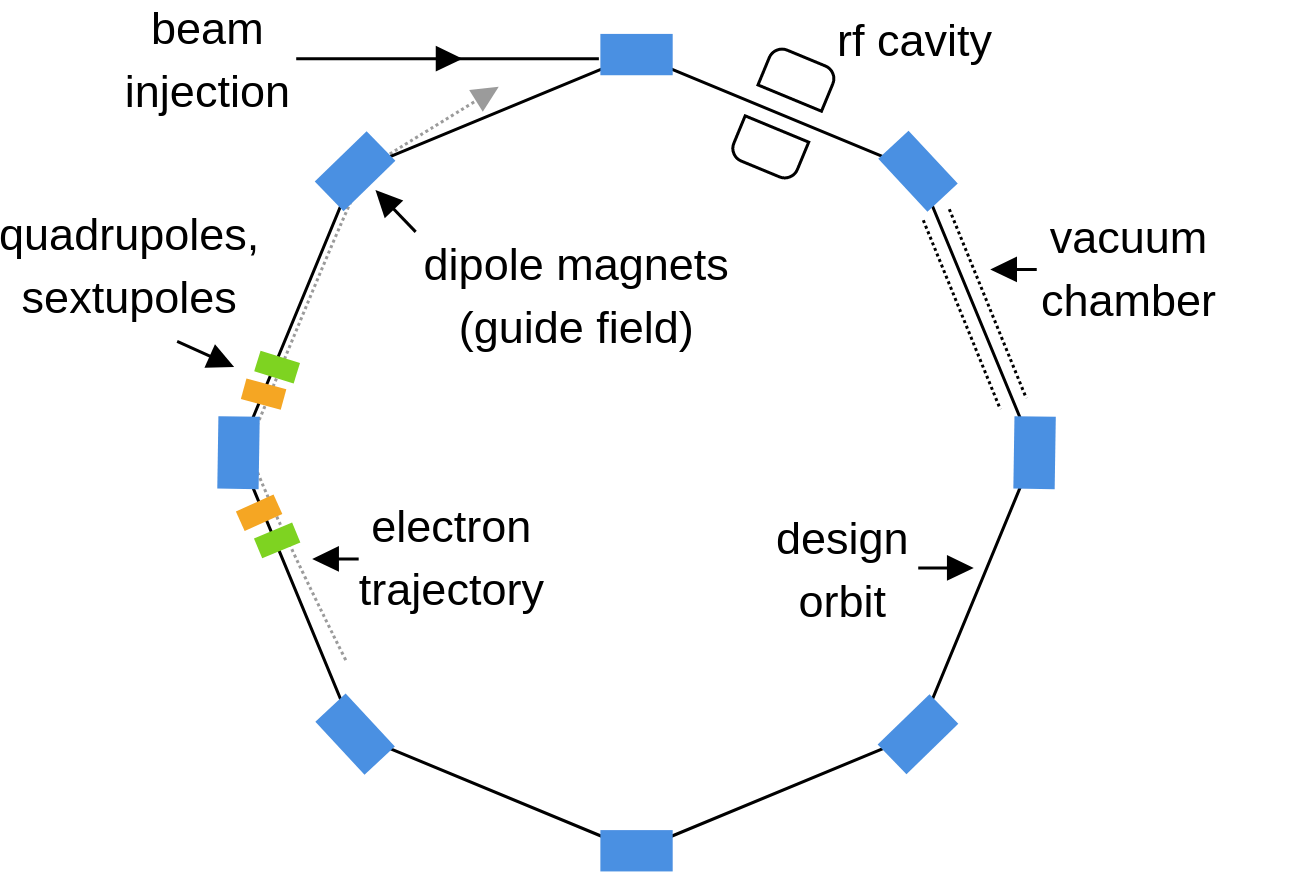
\includegraphics[width=0.4\textwidth]{Images/storage_ring.png}
    \caption{Storage ring typycal configuration. From \cite{sands}}
    \label{fig:storage_ring}
\end{figure}
\todo[inline]{draw my onw figure}
Figure~\ref{fig:storage_ring} sketches the typical design of a storage ring. For the porpose of storing a beam of electrons in closed orbits, magnetic fields defining a closed orbit are necessary. The angular deflections should add up to $2\pi$, and the specification of the beam's operating energy determines the integrated field required for causing the closed orbit deflections.

For providing stability, focusing towards the reference closed orbit is also needed, and can be attained with the introduction of gradient fields whose strengths depend linearly on the tranverse excursions from the reference orbit. Such fields are provided mainly by quadrupole magnets, which are physically realized by specifying  magnetic poles with the shape of truncated hyperbolas.

Sextupole mangets are also usually included in the design of storage rings. The fields they produce is quadratic with transverse displacement and are needed for correction of chromatic errors in the dynamics.
\todo[inline]{add magnets and field profile figures}

\subsection{The coordinate system}
\begin{figure}[htb]
    \centering
    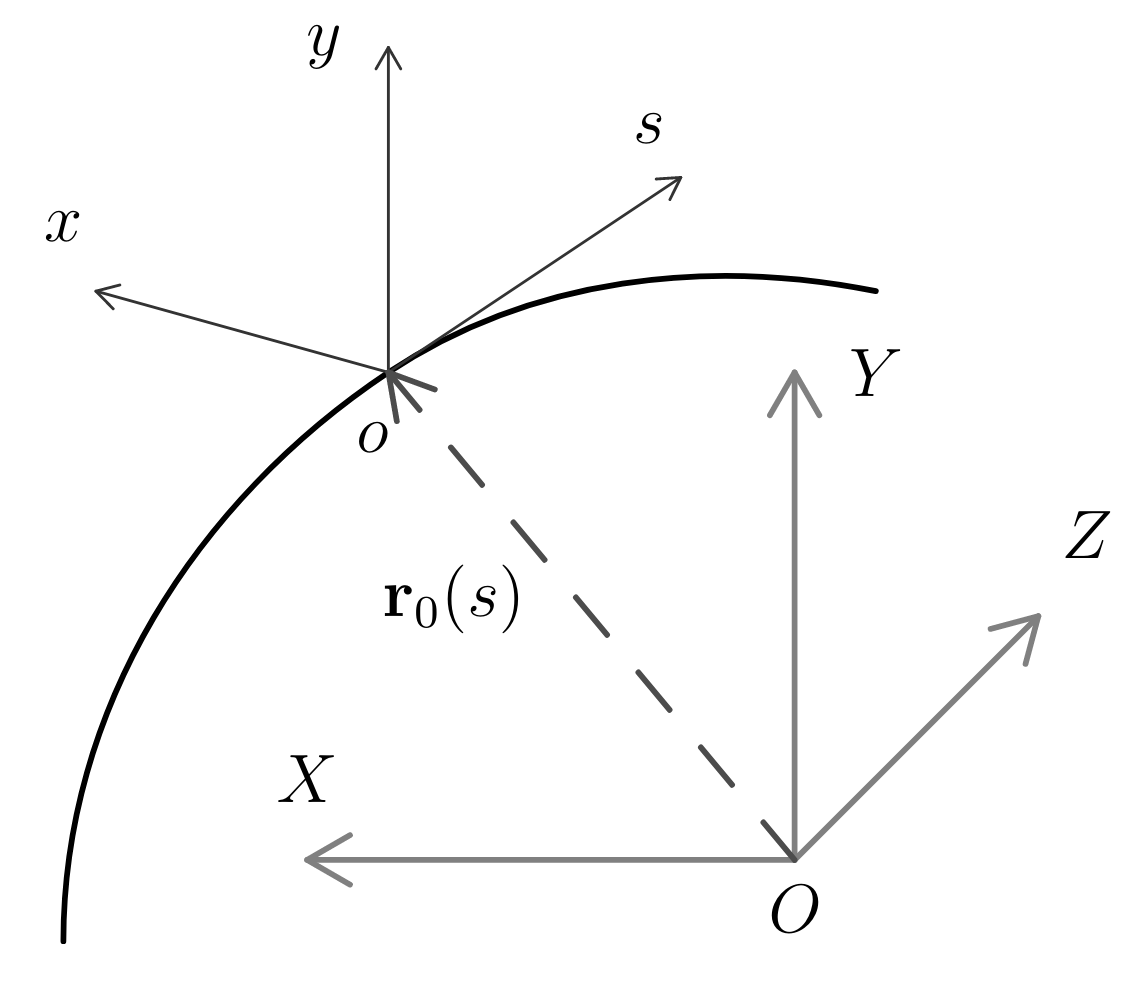
\includegraphics[width=0.6\textwidth]{Images/frenetserret.png}
    \caption{The Frenet-Serret coordinate system. From \cite{huang2019beam}.}
    \label{fig:frenet-serret}
\end{figure}
A convinient coordinate frame to decribe the dynamics in storge rings can be constructed by imagining a reference particle traveling along a curve drawn by the tip of a vector $\vb{r}_0$, as Fig.~\ref{fig:frenet-serret} shows. The particle travels a distance $s$ along the ring, which can be used to parametrize the motion. The triad of direction vectors consists of a vector $\vu{s}$, tangent to the trajectory, a vector $\vu{x}$ normal to it, pointing in the direction at which $\vu{s}$ changes and a vector $\vu{y}=\vu{x}\cross\vu{s}$, bi-normal to the trajectory. This construction leads to a Frenet-Serret reference frame.

Assuming no curvature in the $y$ plane, i.e. that the accelerator defines a curve whose plane is parallel to the ground, then the unit vectors defining the frame can be calculated by\cite{lee}
\begin{equation}
\vu{s}=\dv{\vb{r}_{0}}{s}, \quad \vu{x}=-\rho\dv{\vu{s}}{s}, \quad \vu{y} =  \vu{x}\times\vu{s},
\end{equation}
where $\rho(s) = \norm{\dv*{\vu{s}}{s}}^{-1}$ is the local curvature radius\footnote{For a circular trajectory, $\vb{r}_0 = (R\cos(s/R), R\sin(s/R), 0)$, $ 0\leq s \leq L$ (check), in the cartesian laboratory frame. $\vu{s}=(-\sin(s/R), \cos(s/R), 0)$, $\dv*{\vu{s}}{s} = -R^{-1}(\cos(s/R),\sin(s/R), 0 )$ and $\rho(s)=R$}. The vectors evolve along $s$ as prescribed by the Frenet-Serret equations:
\begin{equation}
\dv{\vu{s}}{s}=-\frac{1}{\rho(s)}\vu{x}, \quad\dv{\vu{x}}{s}=\frac{1}{\rho(s)}\vu{s}, \quad \dv{\vu{y}}{s}=0,
\end{equation}
The frame thus depends solely on the geometry of the specified path. Since the curvature is defined by the dipolar fields $B_0(s)$ in the $y$ direction, then, eq.~\eqref{eq:deflec_angles} leads to
    \begin{equation}
        G(s) \equiv \frac{1}{\rho(s)} = \frac{B_0(s)}{R_0},
        \label{eq:G}
    \end{equation}
where $R_0$ is the rigidity for the beam at the nominal energy.
\subsection{Hamiltonian for the relativistic electron}
The dynamics of relativistic electrons influenced by electromagnetic fields $(\Phi, \vb{A})$ is encapsulated by the Hamiltonian
    \begin{equation*}
        H=\sqrt{m^2c^4+(\vb{P}-q\vb{A})^2c^2}+e\Phi,
    \end{equation*}
 $e$ being the elementary charge and $\vb{P}=\vb{p}+e\vb{A}$ the canonical momentum. The following steps are followed to obtain equations of motion for electrons in the storage ring:
 \begin{itemize}
    \item A canonical transformation to change coordinates is applied in order to describe the motion in terms of the Frenet-Serret frame variables $x$, $y$;
    \item Instead of time $t$, the Hamiltonian and the dynamical variables are described as functions of $s$, the longitudinal position along the ring;
    \item Geometric quantities are used: canonical momenta are the angles $x^\prime = \dv*{x}{s}$ and $y^\prime = \dv*{y}{s}$ with respect to the nominal orbit;
    \item Paraxial approximation: transverse momenta are assumed to be way smaller than longitudinal momentum;
 \end{itemize}

 All of these steps are shown in detail in textbooks such as  Refs.~\cite{lee, wiedemann,  wolski2014beam}. Neglecting RF cavities ($\Phi=0$) and radiation losses, the energy is a constant parameter and the dynamics will consist solely on the transverse degrees of freedom.
  In this 4-dimensional dynamics, the set of canonical variables are $(x,p_{x},y , p_{y})$, where
\begin{equation}\begin{cases} p_{x}= x^\prime(1+\delta),\\p_{y}=y^\prime (1+\delta),\end{cases}\end{equation}
and
\begin{equation}
    \delta = \frac{P-P_{0}}{P_{0}}\approx\frac{E-E_0}{E_0}
\end{equation}
where the ultra-relativistic approximation $E\approx pc$ was used.

Hamilton's equations for the Hamiltonian in the paraxial approximation lead to the equations of motion for 4D dynamics
\begin{equation}
x^{\prime \prime}=-\frac{(1+G x)^{2}}{1+\delta} \frac{B_{y}}{R_0}+G(1+G x),
\quad
y^{\prime \prime}=\frac{(1+G x)^{2}}{1+\delta} \frac{B_{x}}{R_0}
\label{eq:EOMs}
\end{equation}
where $R_0 = p_0/e$ and $G(s)$ defined as in Eq.~\eqref{eq:G}.

Fields influencing the beam are those of dipoles, quadrupoles and sextupoles.
Their functional forms are
\begin{itemize}
    \item Horizontal Dipole:\\
           $$ B_x = 0, \quad B_y = B_0$$
    \item Normal quadrupole\\
          $$B_x = B_1 y, \quad B_y = B_1 x$$
    \item Normal sextupole\\
          $$B_x = B_2xy, \quad B_y = \frac{1}{2}B_2(x^2 - y^2)$$
\end{itemize}
These are the so-called \textit{normal multipole fields}. There also exists \textit{skew multipole fields}, which couple the horizontal and vertical dynamics. We will neglect skew fields and coupling for now.

In the equations of motion, eqs.~\eqref{eq:EOMs}, the magnetic rigidity normalizes all the fields. We define the dipolar, quadrupolar and sextupolar functions by
\begin{equation}
    G(s) = \frac{B_0(s)}{B\rho}, \quad K(s) = \frac{B_1(s)}{B\rho}, \quad S(s) = \frac{B_2(s)}{B\rho}.
    \label{eq:mag_funcs}
\end{equation}

\subsection{Linear Dynamics}
\subsubsection{Linear equations of motion}
Expansion of eqs.~\eqref{eq:EOMs} up to first order in the $x, y, \delta$ variables leads to \cite{sands}
    \begin{equation}
        x^{\prime\prime}+(G^2+K)x=G\delta, \quad
        y^{\prime\prime}-Ky=0.
        \label{eq:linearEOM}
    \end{equation}
    For on-momentum particles, $\delta=0$, both equations reduce to Hill's equations
    \begin{equation}
        u^{\prime\prime}+K_u(s)u = 0,
        \label{eq:Hill}
    \end{equation}
    which are a pair of parametric oscillators for $u=x,y$, with $s$-dependent focusing functions
         $$K_x(s) = G^2(s) + K(s), \quad K_y(s) = - K(s).$$
Motion in the linear approximation thus consists on oscilations around the closed orbit, known as betatron oscillations.
\subsubsection{Pseudoharmonic description}
The solutions for the equations of betatron motion can be cast in a amplitude-phase (WKB) form
\begin{equation}
    u(s) = \sqrt{2\beta_u(s) J_u}\cos(\phi_u(s) + \phi_0),
    \label{eq:pseudo_harmon}
\end{equation}
where $\beta_u(s)$ must satify the boundary value problem
\begin{equation}
    \frac{1}{2}\beta_{u}^{\prime\prime}+\beta_{u} K_u(s) - \frac{1}{\beta_{u}}\qty(\frac{1}{4}\beta_{u}^{\prime 2} + 1 ) = 0, \quad
        \begin{cases}
            \beta_{u}(0) = \beta_{u}(L)\\ \beta_{u}^{\prime}(0) = \beta_{u}^{\prime}(L)
        \end{cases}
    \label{eq:beta_eq}
\end{equation}
and the phase advance must be
    \begin{equation}
        \phi_u(s) = \int_{0}^{s}\frac{1}{\beta_u(\sigma)}\dd\sigma.
   \end{equation}
The betatron functions for the SIRIUS storage ring are shown in Fig.~\ref{betafunc}.
\begin{figure}[htb]
    \centering
    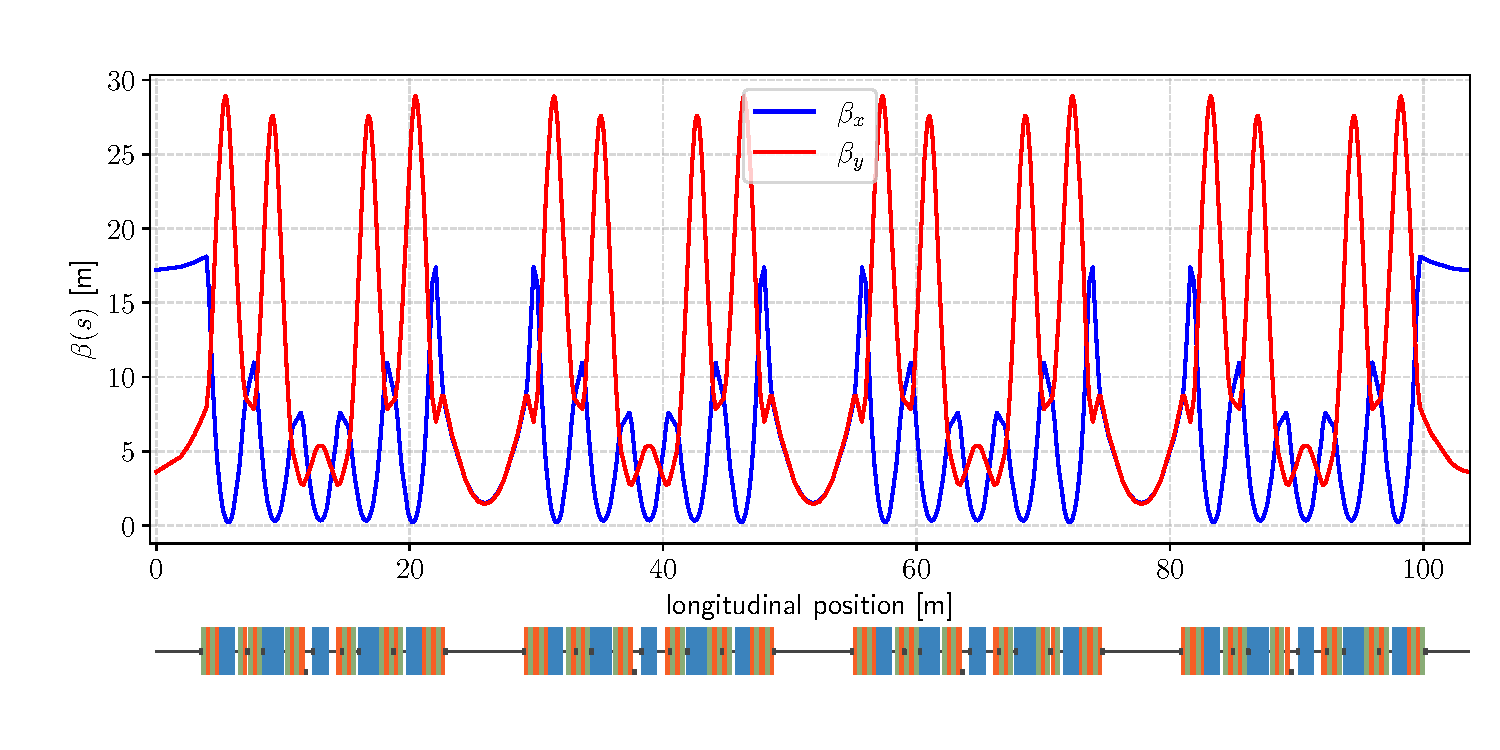
\includegraphics[width=\textwidth]{Images/beta_functions.pdf}
    \caption{Betatron functions for the SIRIUS storage ring. Colored blocks represent the magnets of the accelerator lattice: blue for dipoles, orange for quadrupoles and green for sextupoles. The ring has a 5-fold symmetry, with the lattice and betatron function repeating the same pattern shown above five times up to $s=518~\unit{m}$}
    \label{betafunc}
\end{figure}

An important feature of the dynamics is the \textit{tune}: the phase advance per ring revolution
\begin{equation*}
    \nu_u=\frac{1}{2\pi}\int_{s}^{s+L}\frac{\dd \sigma}{\beta_u(\sigma)}\equiv\frac{1}{2\pi}\oint\frac{\dd s}{\beta_u(s)}.
\end{equation*}
The analysis of perturbations and nonlinearities shows that the tunes are a critical variables in determining the beam's response to perturbations. More specifically, the tunes impact over disturbances amplifiction factors, which are greatest when tunes are close to integer numbers.

% SIRIUS ring has tunes $(\nu_x, \nu_y)=(49.08, 14.14)$ which are very close to integers. It is desired to increase the tunes fractional parts to reduce orbit amplification factors. This is the reason why injection efficiency optimzation runs have also been carried in different machine tunes.
\subsubsection{Turn-by-turn motion}
In the $u, u^\prime$ phase space, the quasi-periodic motion traces out ellipses. This can be verified by calculating the derivative
    \begin{equation}
        u^{\prime}(s) = - \sqrt{\frac{2J_u}{\beta_u}}\qty[\sin(\phi_u(s) + \phi_0) + \frac{1}{2}\beta_u^\prime(s)\cos(\phi_u(s) + \phi_0)],
        \label{eq:uprime}
    \end{equation}
    defining $\alpha_u = \frac{\beta_u^\prime}{2}$  and $\gamma_u = \frac{(1+\alpha_u^2)}{\beta_u}$ and checking that $u, u^\prime$ satify the quadratic form
    \begin{equation}
        2J_u=\gamma_u u^{2}+2\alpha_u u u^{\prime}+\beta_u u^{\prime2}.
     \end{equation}

The ellipse properties are defined by the $\beta(s), \alpha(s)$ and $\gamma(s)$ functions, also known as Courant-Snyder (C-S) parameters or Twiss parameters. Tracking a particle's transverse position and momenta for several turns at some fixed point along the ring results in the ellipse with shape specified by the C-S parameters. Since the parameters are functions of the position $s$, then, at each point along the accelerator, the Poincaré Section $u, u^\prime$ displays a different ellipse for each point.

 Since the phase advance over a turn is $2\pi \nu+\phi_0$, the phase advance after the $j$-th turn is $2\pi\nu j+\phi_0$, and thus
 sampling the transverse motion at a fixed $s=s_0$ position reveals a harmonic displacement
\begin{equation}
    u_j(s_0)=\sqrt{2\beta_u(s_0) J_u}\cos(2\pi\nu_u j+\phi_u(s_0)).
    \label{eq:TbT_motion}
\end{equation}
% Time of flight during a complete turn is $L/c$ so, for the $j$th turn, $t_j=\frac{L}{c} j$. With a revolution frequency of $\omega_r=2\pi/(L/c)$, we see that $2\pi j= \omega_r t_j$. As a function of the time elapsed over the $j$ turns, the displacements reads
% \begin{equation}
%     x_j=\sqrt{2\beta_0J}\cos(\omega_r\nu t_j+\phi_0).
% \end{equation}
\begin{figure}[htb]
    \centering
    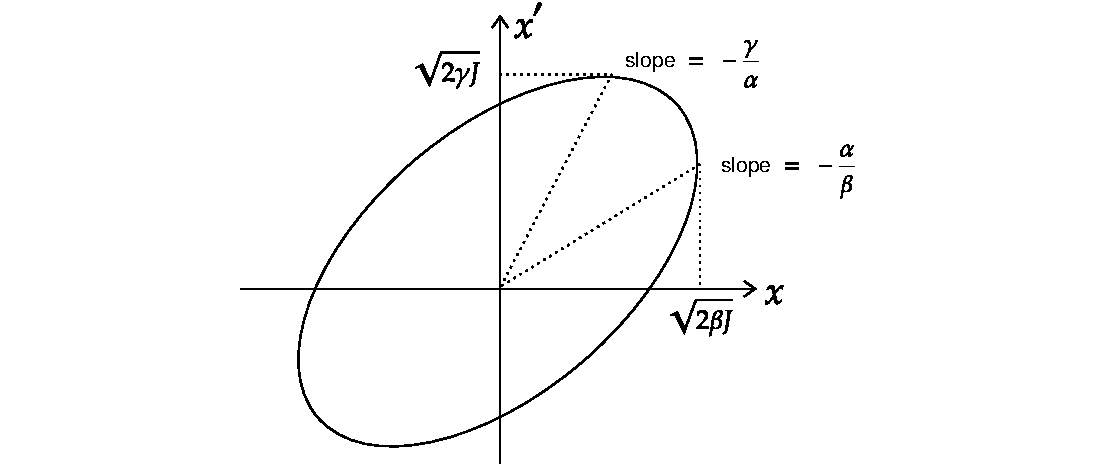
\includegraphics[width=0.5\textwidth]{Images/ellipse}
    \caption{Phase space ellipse traced by tur-by-turn (TbT) motion in the $(x,p_x)$ phase space. Optics functions determine the principal axes ratios and the inclination of the ellipse at each longitudinal position along the ring. From \cite{wolski2014beam}.}
    \label{ellipse}
\end{figure}
\subsubsection{Dispersion}
The equation of motion for off-momentum particles in the horizontal plane is the non-homogeneous Hill's equation. The solution consists on the linear combination of the homogeneous solutions in the phase-amplitude form plus the particular solution: $x=x_\beta+ x_\delta = x_\beta+ \eta(s)\delta $ where $\eta(s)$ is the \textit{dispersion function}, satisfying
    \begin{equation*}
        \eta^{\prime\prime}+(G^2+K)\eta=G,\quad
        \begin{cases}
            \eta(0) = \eta(L),\\
            \eta^\prime(0) = \eta^\prime(L).
        \end{cases}
    \end{equation*}
    The periodicity in the $\eta(s)$ function is required if we want to interpret $\eta$ as closed orbit per momentum deviation. Thus, off-momentum particles perform betatron oscillations around a dispersive orbit. The dispersion function for the SIRIUS storage ring is shown in Fig.~\ref{dispersion_func}
    \begin{figure}[htb]
        \centering
        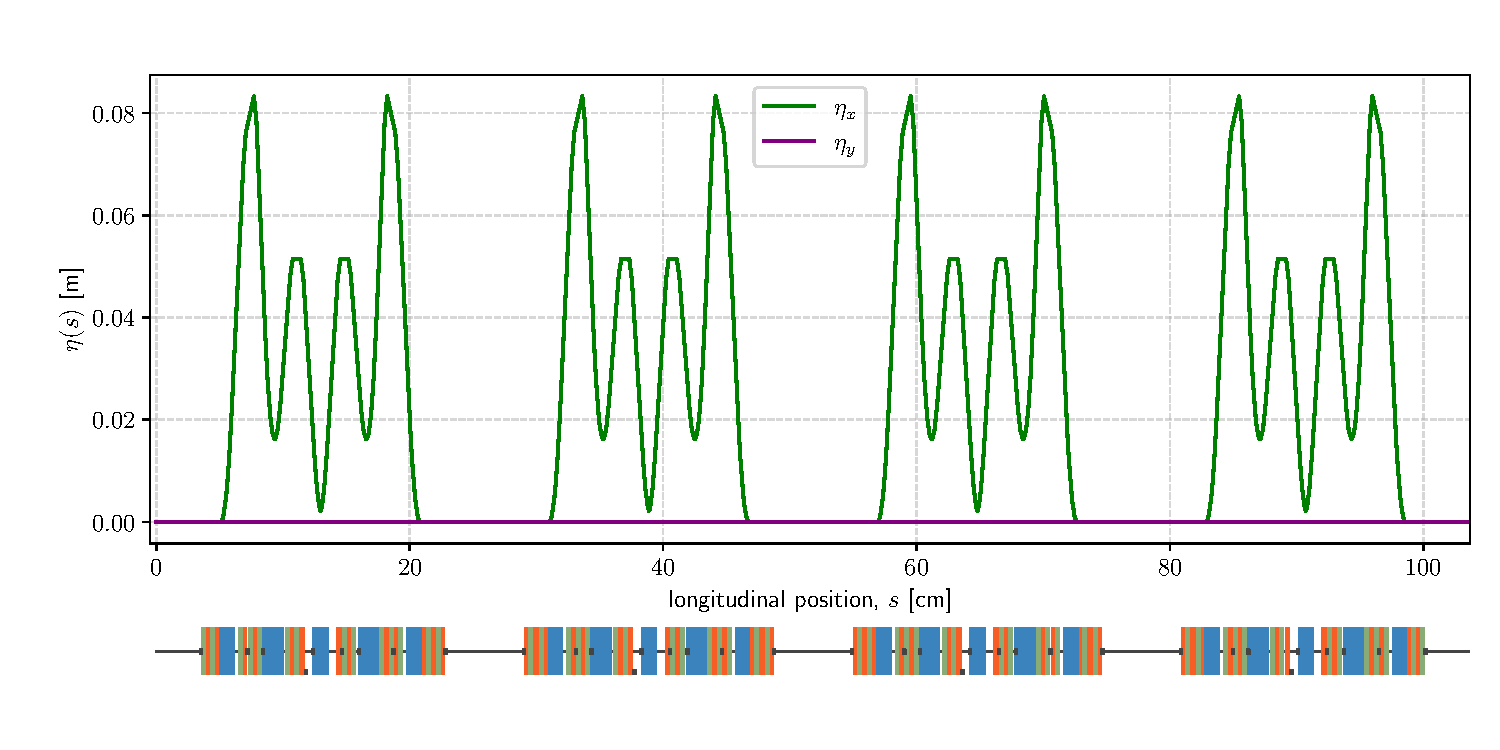
\includegraphics[width=\textwidth]{Images/dispersion.pdf}
        \caption{Dispersion fucntion for SIRIUS superperiod.}
        \label{dispersion_func}
    \end{figure}
\subsubsection{Field Errors}
    % The dipolar contributions promote additional bendgin and thud disturb the design orbit. Assuming the perturbations are not strong enough to kill the beam, a distorted closed orbit must exist. To find it we need to find the coordinates along the ring which are mapped to themselves after a complete revolution. That is, we must find the fixed point $\vb{X}_{\text{co}}$ of the disturbed one-turn map:
    % \begin{equation}
    %     \vb{X}_{\text{co}} = \mathbf{M} \vb{X}_{\text{co}} + \boldsymbol{\Delta}
    % \end{equation}
    % where $\boldsymbol{\Delta} = (0, \theta)^\intercal$, $\theta = B_y \Delta s / B\rho$ for the $(x, x^\prime)$ slice of the closed orbit, $\theta = B_x \Delta s / B\rho$ for the $(y, y^\prime)$. Solving for the closed orbit we find
    % \begin{equation}
    %     \vb{X}_{\text{co}} = (\mathbf{I} - \mathbf{M})^{-1}\boldsymbol{\Delta}.
    % \end{equation}
    % Using the Courant-Snyder parametrization for the one-turn map at the point $s_0$ immediately downstream the perturbation leads to
    % \begin{equation}
    %     \vb{X}_\text{co} = \frac{\theta}{2\sin\pi\nu}\mqty(\beta_0 \cos\pi\nu \\ \sin\pi\nu - \alpha_0 \cos\pi\nu).
    % \end{equation}

    In the presence of additional dipolar and quadrupolar fields $\Delta G$ and $\Delta K$, respectively, the orbit and focusing are changed. Assuming these are small perturbations and not strong enough to kill the beam, we can evluate the disturbances to the unperturbed dynamics.
    The closed orbit distortion due to a single dipole error $\Delta G$ reads
    \begin{equation}
        x_{\text{co}}(s) = \frac{\sqrt{\beta(s)\beta_0}}{2\sin\pi\nu}\Delta G\cos(|\phi(s)-\phi_0| - \pi\nu).
        \label{eq:cod}
    \end{equation}
    For a distribution $\Delta G(s)$ of dipolar perturbations along the ring, we sum over the contributions, and obtain the total disturbance
    \begin{equation}
        x_{\text{co}}(s) = \frac{\sqrt{\beta(s)}}{2\sin\pi\nu}\int_{s}^{s+L} \Delta G(\sigma)\sqrt{\beta(\sigma)}\cos(\pi\nu + \phi(s) - \phi(\sigma))\dd \sigma.
        \label{eq:cod_dist}
    \end{equation}
    % Knowledge of the beam-response to perturbations allows for the inversion of the problem. We can use specified small dipole kicks to correct the orbit, bringing it closer to the nominal one. These small dipole fields are generated by corrector magnets (CM's) abd orbit correction consists on linear problem of seeking CMs strength that minimze orbit distortions.

    % A quadrupole error can be represented by a thin-lens quadrupole transfer matrix \cite{Courant:1958wbj}
    % \begin{equation}
    %     \mathbf{M}_q = \mqty(1 & 0 \\ -k\Delta s & 1),
    %  \end{equation}
    %  so that, immediately downstream the error, the transfer matrix reads $\mathbf{M} = \mathbf{M}_q \mathbf{M}_0$. As a consequence, the optics deviates from the nominal optics. More notouriously, the beta and the phase advances, and thus tune, changes.

    %  The phase advance over a turn, $\phi$, is related to the trace of the one-turn transfer matrix $\mathbf{M}$ as $\cos\phi = 2 \tr \mathbf{M}$. Using the CS parametrization for $\mathbf{M}$, performing the multiplication $\mathbf{M}_q \mathbf{M}_0$ and calcualting the trace leads to
    %  \begin{equation}
    %     \cos \phi - \cos\phi_0 = - \frac{1}{2} k(s)\Delta s \beta_0 \sin\phi_0.
    %  \end{equation}
    %  In a linear approximation (if $\sin \phi_0$ is not near zero) $\Delta(\cos \phi) = \cos \phi - \cos\phi_0 \approx \Delta \phi\dv*{(\cos \phi)}{\phi}$ so the tune-shift due to a single thin-lens quadrupole error is

    As for gradient errors, focusing is changed, which leads to changes in the beta function and phase advance. The tune-shift as a consequence of a gradient error present ``during" a small extent $\Delta s$ along the ring is
         \begin{equation}
        \Delta \nu \approx \frac{1}{4\pi} \beta_0 \Delta K \Delta s.
        \label{eq:delta_nu}
     \end{equation}
     Again, for a distribution of errors we sum over the ring:
     \begin{equation}
        \Delta \nu \approx \frac{1}{4\pi}\oint \beta(s) \Delta K(s) \dd s.
        \label{eq:delta_nu_dist}
    \end{equation}
    %  Besides calculating the tune-shift, the resulting transfer-matrix for the lattice with errors allows for the identification of the new optics $\alpha, \beta, \gamma$, which can then be propagated to anywhere in the ring. In particular we can identify $\beta$ and its fractional deviation from the nominal value along $s$, a parameter known as \textit{beta-beating}
    Is also possible to show tha the the relative beta-function error, known as beta-beating, reads
     \begin{equation}
        \frac{\Delta \beta(s)}{\beta(s)} = - \frac{1}{2\sin(2\pi\nu_0)}\int_{s}^{s+L}\Delta K(\sigma)\cos(2\phi(\sigma)-2\phi(s)-\phi_0)\dd\sigma.
        \label{eq:beta_beat}
     \end{equation}
\subsubsection{Chromaticity}
Energy deviations affect not only the closed orbit by means of the dispersion effect. A more/less energetic beam has higer/lower rigidity and thus is focused differently when passes through quadrupoles.
%  This chromatic aberration effect needs to be corrected, which can be attained with the insertion of geometric aberrations provided by sextupolar fields.
% As for the higher order effect on the focusing, also known as chromatic effect, we consider the motion in a straight section under a gradient, so that there is no non-homogeneous term in the horizontal equation. The equation of motion considering $x\delta $ terms reads
% \begin{equation}
%     x^{\prime\prime}+(K_x+\Delta K_x)x=0
% \end{equation}
% \begin{equation}
%     y^{\prime\prime}+(K_y+\Delta K_y)y=0
% \end{equation}
% where $K_x=h^2+K_1$, e $K_y=-K_1$ and

Expanding the equations of motion, \eqref{eq:EOMs}, for off-energy particles up to the order of terms $u\delta$ ($u=x,y$) gives the additional higher-order gradient terms
\begin{equation}
    \Delta K_x = -(K_1+2G^2)\delta \approx K_x\delta
\end{equation}
\begin{equation}
    \Delta K_y = K_1\delta = -K_y\delta
\end{equation}
This means there exists an energy-dependent tune-shift effect, which, using eq.~\eqref{eq:delta_nu_dist}, reads
% The result is that an off-momentum partcile sees a different optics along the ring: different beta function and different phase advance. Thus, it deviates from nominal operation conditions, specially in the tunes, inducing the tune-shifts
\begin{equation}
    \Delta \nu _i \approx -\frac{1}{4\pi}\oint\beta K_i \delta \dd{s},
    \label{eq:energy_delta_tune}
\end{equation}
for the $i=x,y$ planes.

We can define the \textit{linear chromaticity} in the $i=x,y$ direction as energy error-induced tune-shift $\Delta \nu_i$ per energy deviation $\delta$
\begin{equation}
    \xi_i=\dv{\nu_i}{\delta}.
\end{equation}
This uncorrected chromaticity is also called natural chromaticity. Using expression \eqref{eq:energy_delta_tune} for the tune-shift, the natural chromaticity reads
\begin{equation}
\xi_{i, \text {nat }} \approx-\frac{1}{4 \pi} \oint K_i \beta_i \dd{s}.
\end{equation}

To correct this chromatic effect,  we need to introduce sextupolar fields in the lattice, specifically in the dispersive regions. In such regions, off-energy particles should have a deviation from the design closed orbit. Their position reads $x(s)=x_{\beta}(s)+\eta(s) \delta$, where $x_{\beta}(s)$ consists on the betatron oscillations. Since sextupolar fields are of the form
$$B_{x}=B_{2} x y, \quad B_{y}= \frac{B_{2}}{2}(x^{2}-y^{2}),$$
then, the off-momentum particles ``see" the fields
$$B_{x}=B_{2}(x_\beta y + \eta \delta y), \quad B_{y}=\frac{B_{2}}{2}({x_\beta^{2}-y^{2}})+B_2 x_\beta \eta \delta + \frac{B_2}{2}(\eta \delta)^2,$$
So, to lowest, order they feel a dipolar perturbation and the gradient error
$$\Delta K_{x,y}(\delta)=\pm S\eta \delta.$$
Considering both the energy deviation-induced gradient errors and the sextupole gradient effect, we have a total error $\Delta K = (K - S\eta)\delta$ in eq.~\eqref{eq:delta_nu_dist}. The chromaticity in a lattice with sextupoles thus reads
\begin{equation*}
    \xi_{x,y}=\mp \frac{1}{4\pi}\oint\beta_{x,y}(K_{x,y}- S\eta)\dd s,
\end{equation*}
which depends linearly on sextupole strengths, allowing for the correction of chromaticity to specified values. The cost of correcting chromaticity is the insertion of perturbations and nonlinearities in the dynamics.

% More broadly speaking, the energy deviations induce the beam to see a completely different optics. The contributions to the changes can be of any order. For instance
% \begin{equation}
%     \Delta \nu = \xi^{(1)} \delta + \xi^{(2)}\delta ^2+ \dots
% \end{equation}
% similarly
% \begin{equation}
%     \Delta \beta(s, \delta) = \beta^{(1)}(s) \delta + \beta^{(2)}(s) \delta^2 + \dots
% \end{equation}
\subsection{Nonlinear Dynamics and Perturbations}
\subsubsection{Action Angle Variables}
Betatron motion of equation~\eqref{eq:Hill} can be obtained as Hamilton's equations for the effective Hamiltonian
\begin{equation}
    \mathcal{H}=\frac{1}{2}u^{\prime2}+\frac{1}{2}K_u(s)u^2.
\end{equation}
A transformation $(u,u^\prime)\to(\psi, J)$ to Action-angle variables is implicitly implemented by the generating function
\begin{equation}
    F_1(u,\phi_u)=\int{u}^\prime\dd{{u}}=\frac{u^2}{2\beta_u}\qty(\tan \phi_u-\frac{\beta_u^\prime}{2}).
\end{equation}
The action variable reads
\begin{equation}
    J_u=-\pdv{F_1}{\phi_u} = \frac{u}{2\beta_u}\sec^2\phi_u = \frac{1}{2\beta_u}[u^2 + (\beta_u u^\prime + \alpha_u u^2)],
    \label{eq:action}
\end{equation}
from which we recover the pseudo-harmonic form $u=\sqrt{2\beta_u J_u}\cos(\phi_u(s)+\phi_0)$. This justifies our choice for the amplitude constant in the pseudo-harmonic description.

In the $J,\phi$ variables, the new hamiltonian is $H_0(\phi, J)$,  given by
\begin{equation}
    H_0=\mathcal{H}+\pdv{F_1}{s} = \frac{J}{\beta}.
\end{equation}
Performing the change to action-angle variable in both the horizontal and vertical planes we find the new Hamiltonian for 4D dynamics
\begin{equation}
    H_0= \frac{J_x}{\beta_x} +  \frac{J_y}{\beta_y},
\end{equation}
and Hamilton's equations read
\begin{equation}
    \phi_u^\prime = \frac{1}{\beta_u(s)},\qquad J_u^\prime=0.
\end{equation}
\subsubsection{Perturbations and tune-shifts}
Linear motion is integrable, since it can be written in terms of the action variable only (angle-independent Hamiltonian). This leads to the action variable being a constant of motion, and the phase advance behaving just as the pseudo-harmonic motion anticipated.

Linear motion, though, is only a useful first approximation. In reality, in an storage ring, there are higher order multipole magnets, such as sextupole magnets, and also multipole, alignement and excitation errors, all acting as perturbations to linear motion. Generically referring to perturbations as $V(J, \phi)$, we can write the perturbed motion Hamiltonian
\begin{equation}
    H(J,\phi) =H_0 + V(J,\phi).
\end{equation}
Hamilton's equations read
\begin{equation}
\phi_u^\prime = \frac{1}{\beta_u(s)}+\pdv{V(J,\phi)}{J_u}, \quad J_u^\prime = \pdv{V(J,\phi)}{\phi_u}.
\end{equation}
Since the tunes consist on the phase advance per revolution, we immediately see that the presence of perturbations leads to tune-shifts.

Generically, the tunes can be expressed in terms of the tune-shifts as
$$\nu_0 = \nu_{u0} + \xi_u(\delta) \delta + \alpha_{uu} J_u + \alpha_{uv} J_v$$
where $\xi_u$ represents the momentum-dependent tune-shifts (higher order chromaticity), and the other components consist on the amplitude-dependent tune-shifts, up to first order in the actions.


\subsubsection{Ressonances}
4D linear unperturbed motion consists on the motion of two uncoupled parametric oscillators. The phase-space is diffeomorphic to the 2-Torus, $\mathbb{T}^2$, and there are an infinite number of such tori, corresponding to the different initial conditions $J_u$. Canonical perturbation theory applied to the perturbed motion fails to converge whenever the ratio of tunes is sufficiently rational. The Poincare-Birkhoff theorem states that under such conditions, almost all the periodic phase-space orbits disappear. An even number of tori survives, half of which are stable and half unstable. Unstable motion in a storage ring can eventually lead to beam loss.

The condition for sufficiently rational tunes can be expressed as
    $$m\nu_x + n\nu_y = \ell,$$
    for $n, m, \ell\in\mathbb{Z}$, and defines the lines in tune-space in which perturbation theory fails and motion can become unstable. These are resonance lines and $|n|+|m|$ is the order of the resonance. Figure~\ref{resons} shows resonance lines for the resonances up to second, third and fourth order respectively. First order resonances can be excited by dipolar fields, 2nd order resonances can be excited by quadrupole fields and 3rd order resonances can be driven by sextupolar fields.
\begin{figure}[thb]
    \centering
    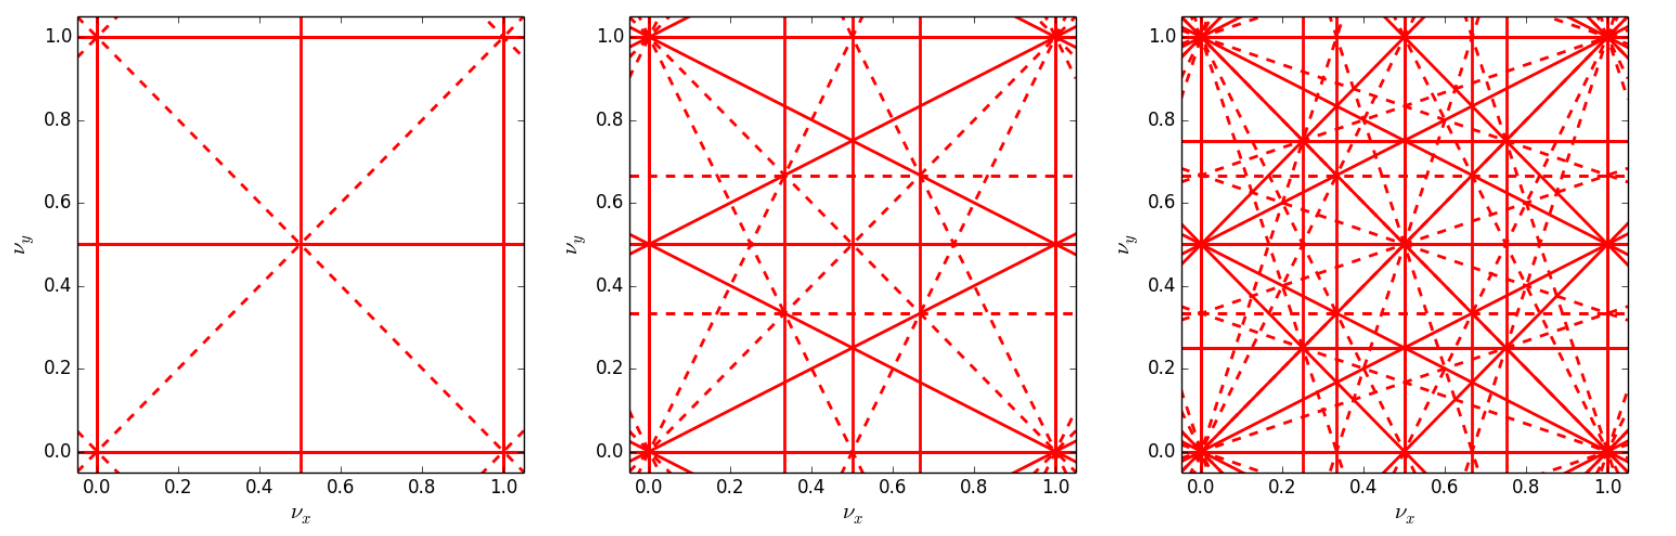
\includegraphics[width=\textwidth]{Images/tunes.png}
    \caption{Resonance lines in tune space up to 2nd, 3rd and 4th order, respectively.}
    \label{resons}
\end{figure}
\subsubsection{Dynamic Aperture}
    Nonlinear dynamics can become sensitive to initial conditions when the amplitudes are large. Because of the tune-shfits, specially the amplitude-dependent tune shifts, the tunes can wander in tune space, eventually crossing resonance conditions that may lead to instabilities, chatotic motion and beam loss. The dynamics can impose limitations to the maximum transverse deviations in which the beam can oscillate while displaying regular and bounded motion. This is a dynamic restriction to the motion known as the \textit{dynamic aperture}.

    Exceeding the dynamic aperture eventually leads to beam loss. During injection of the beam, if the transverse offsets are larger than the dynamic aperture, the beam is not captured into the storage ring. This is specially important for off-axis injection, such as in the case for SIRIUS.
